\documentclass[a4paper,11.5pt]{article} % тип документа


%%%Библиотеки
	%\usepackage[warn]{mathtext}	
	\usepackage[T2A]{fontenc} % кодировка
	\usepackage[utf8]{inputenc} % кодировка исходного текста
	\usepackage[english,russian]{babel} % локализация и переносы
	\usepackage{caption}
	\usepackage{listings}
	\usepackage{amsmath,amsfonts,amssymb,amsthm,mathtools}
	\usepackage{wasysym}
	\usepackage{graphicx}%Вставка картинок правильная
	\usepackage{float}%"Плавающие" картинки
	\usepackage{wrapfig}%Обтекание фигур (таблиц, картинок и прочего)
	\usepackage{fancyhdr} %загрузим пакет
	\usepackage{lscape}
	\usepackage{xcolor}
	\usepackage[normalem]{ulem}
	\usepackage{hyperref}

%%%Конец библиотек




%%%Настройка ссылок
	\hypersetup
	{
		colorlinks=true,
		linkcolor=blue,
		filecolor=magenta,
		urlcolor=blue
	}
%%%Конец настройки ссылок


%%%Настройка колонтитулы
	\pagestyle{fancy}
	\fancyhead{}
	\fancyhead[L]{Вопрос по выбору}
	\fancyhead[R]{Талашкевич Даниил, группа Б01-009}
	\fancyfoot[C]{\thepage}
%%%конец настройки колонтитулы



							\begin{document}
						%%%%Начало документа%%%%


%%%Начало титульника
\begin{titlepage}

	\newpage
	\begin{center}
		\normalsize Московский физико-технический институт \\(госудраственный 			университет)
	\end{center}

	\vspace{6em}

	\begin{center}
		\Large Лабораторная работа по электричеству\\
	\end{center}

	\vspace{1em}

	\begin{center}
		\large \textbf{Свободные колебаний в электрическом контуре [3.2.4]}
	\end{center}

	\vspace{2em}

	\begin{center}
		\large Талашкевич Даниил Александрович\\
		Группа Б01-009
	\end{center}

	\vspace{\fill}

	\begin{center}
	Долгопрудный \\2021
	\end{center}
	
\end{titlepage}
%%%Конец Титульника



%%%Настройка оглавления и нумерации страниц
	\thispagestyle{empty}
	\newpage
	\tableofcontents
	\newpage
	\setcounter{page}{1}
%%%Настройка оглавления и нумерации страниц


					%%%%%%Начало работы с текстом%%%%%%

\section{Аннотация}

\subsection{Цель работы}
\begin{enumerate}
\item   Исследование свободных колебаний в электрическом контуре.
\end{enumerate}

\subsection{В работе используются:}
\begin{itemize}
    \item Генератор импульсов
    \item электронное реле
    \item магазин сопротивлений
    \item магазин емкостей
    \item катушка индуктивности
    \item электронный осциллограф
    \item универсальный измерительный мост 

\end{itemize}

\subsection{Теоретическое вступление и модель}

В работе планируется:

\begin{enumerate}
    \item Исследовать зависимость периода свободных колебаний контура от емкости. Согласно теории, зависимость должна иметь вид (Формула Томпсона):

\begin{equation}
    T = 2\pi \sqrt{LC} \quad
\end{equation}
    

    где $T$ - период колебаний, $L$ и $C$ - индуктивность и емкость контура соответственно.

    Период планируется измерять с помощью осциллографа.

    \item Исследовать зависимость логарифмического декремента затухания от сопротивления. \\ Расчет логарифмического декремента затухания будет производиться по следующей формуле:

\begin{equation}
	\lambda = \frac{1}{n} \ln\frac{W_k}{W_{k+n}} \quad    
\end{equation}
    

    где $W_i$ - энергия контура после i-того колебания.

    Энергию контура планируется высчитывать используя напряжение на конденсаторе, которое в свою очередь, измеряется с помощью осциллографа. \\

    
Согласно теории, логарифмический декремент затухания пропорционалени сопротивлению
\begin{equation}
	\lambda \propto R
\end{equation}
    
    \newpage

    \item Определить критическое сопротивление. Критическое сопротивление вычисляется по формуле:

\begin{equation}
	R_\text{кр} = 2\sqrt{\frac{L}{C}}
\end{equation}
   

    \item Определить добротность контура. Добротность планируется вычислить двумя способами, с последующим сравнением результатов. \\

    Первый способ - Через формулу для логарифмического декремента затухания. \\
    Второй способ - используя параметры контура R, L, C. \\[0.1cm]

    Формула для вычисления добротности через логарифмический декремент затухания:
\begin{equation}
	Q = \frac{\pi}{\lambda}
\end{equation}
    Формула для вычисления добротности с использованием параметров контура
\begin{equation}
 	Q = \frac{1}{R} \sqrt{\frac{L}{C}}
\end{equation}

\end{enumerate}

\section{Экспериментальная установка}

Схема установки представлена на рисунке 1.

\begin{center}

    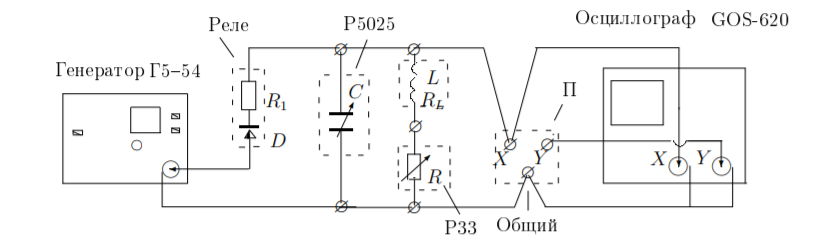
\includegraphics[scale=0.6]{324_scheme.png} \\
    \textit{Рис. 1. Схема установки}

\end{center}

\section{Ход работы}


\subsection{Снятие данных}

XXX.

\subsection{Аппроксимация полученных данных}

XXX

\subsection{Графики и таблицы}

XXX

\subsection{Вывод}

XXX

\section{Список используемой литературы}

\begin{itemize}
\item Гладун А. Д. Лабораторный практикум по общей физике. Термодинамика и молекулярная физика\\

\item \href{https://mipt.ru/education/chair/physics/S_II/lab/}{Описание лабораторных работ на кафедре общей физики МФТИ}
\end{itemize}


\newpage

					\end{document}